%\begin{frame}{EPAM}
%  \begin{center}
%    
\includegraphics[height=3.3cm]{epam}
%  \end{center}
%\end{frame}

\begin{frame}{}
	\begin{columns}
		\column{0.7\textwidth}
		\Huge
		\center{Developers!\\Developers!\\Developers!\\}
		\column{0.3\textwidth}
		\center
\includegraphics[height=4cm]{steve_ballmer}
	\end{columns}
\end{frame}


\begin{frame}
	\frametitle{Курсы Linux от Epam}

	\begin{block}{Цели}
		\begin{itemize}
			\item Увеличение популярности GNU/Linux среди программистов
			\item Воспитание потенциальных сотрудников
		\end{itemize}
	\end{block}

	\pause

	\begin{block}{Целевая аудитория}
		\begin{itemize}
			\item Студенты технических специальностей
			\item Программисты, желающие освоить работу в ОС Linux
		\end{itemize}
	\end{block}

	\begin{block}{Требования к кандидатам}
		\begin{itemize}
			\item Уметь программировать, под любую платформу.
		\end{itemize}
	\end{block}

\end{frame}

\begin{frame}
	\frametitle{Программа курсов}

	\begin{block}{Командная строка -- важнейший инструмент понимания процесса разработки}
		\begin{itemize}
			\item Представление об архитектуре GNU/Linux дистрибутива
			\item Введение в shell-программирование
			\item Классические средства разработки, отладки и оптимизации
		\end{itemize}
	\end{block}
\end{frame}

\begin{frame}
	\frametitle{Формат проведения занятий}

	\begin{block}{Принципы}
		\begin{itemize}
			\item Лекторы? Учителя? {\bf NO WAY!!!} \newline 
				Разработчики для разработчиков! 
			\item Небольшая группа изучающих
			\item Балланс между теорией и практикой
		\end{itemize}
	\end{block}

	\begin{block}{Место проведения}
		\begin{itemize}
			\item Совместная лаборатория Epam-БГУИР 
		\end{itemize}
	\end{block}

\end{frame}

\subsection[2012]{Курс 2012-2013}

\begin{frame}
  \frametitle{Первый набор (2012-2013)}
  \begin{columns}
    \column{0.5\textwidth}
	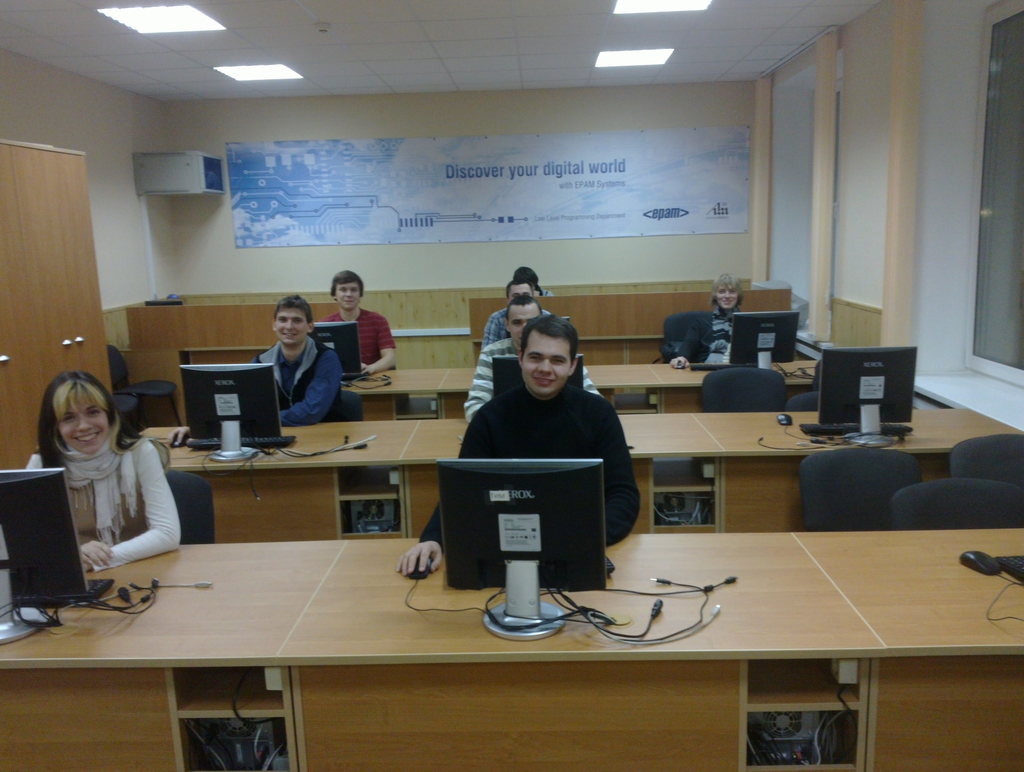
\includegraphics[width=\textwidth]{epam-evm_lab512}

    \column{0.5\textwidth}
	\begin{block}{Немного статистики}
		\begin{itemize}
			\item Подано заявок -- {\bf 39} человек
			\item После первоначального отбора: {\bf 16} человек
				\begin{itemize}
					\item из них {\bf 4} -- сотрудники Epam
				\end{itemize}
			\item Получили сертификаты -- {\bf 13} человек
			\item Устроились на Epam, как Linux-разработчики -- {\bf 4} человека
            \item Планировали 48 часов
            \pause
			\begin{itemize}
    				\item[--] Получилось 66 часов
			\end{itemize}
		\end{itemize}
	\end{block}
  \end{columns}
\end{frame}

\begin{frame}
  \frametitle{Успех!}
  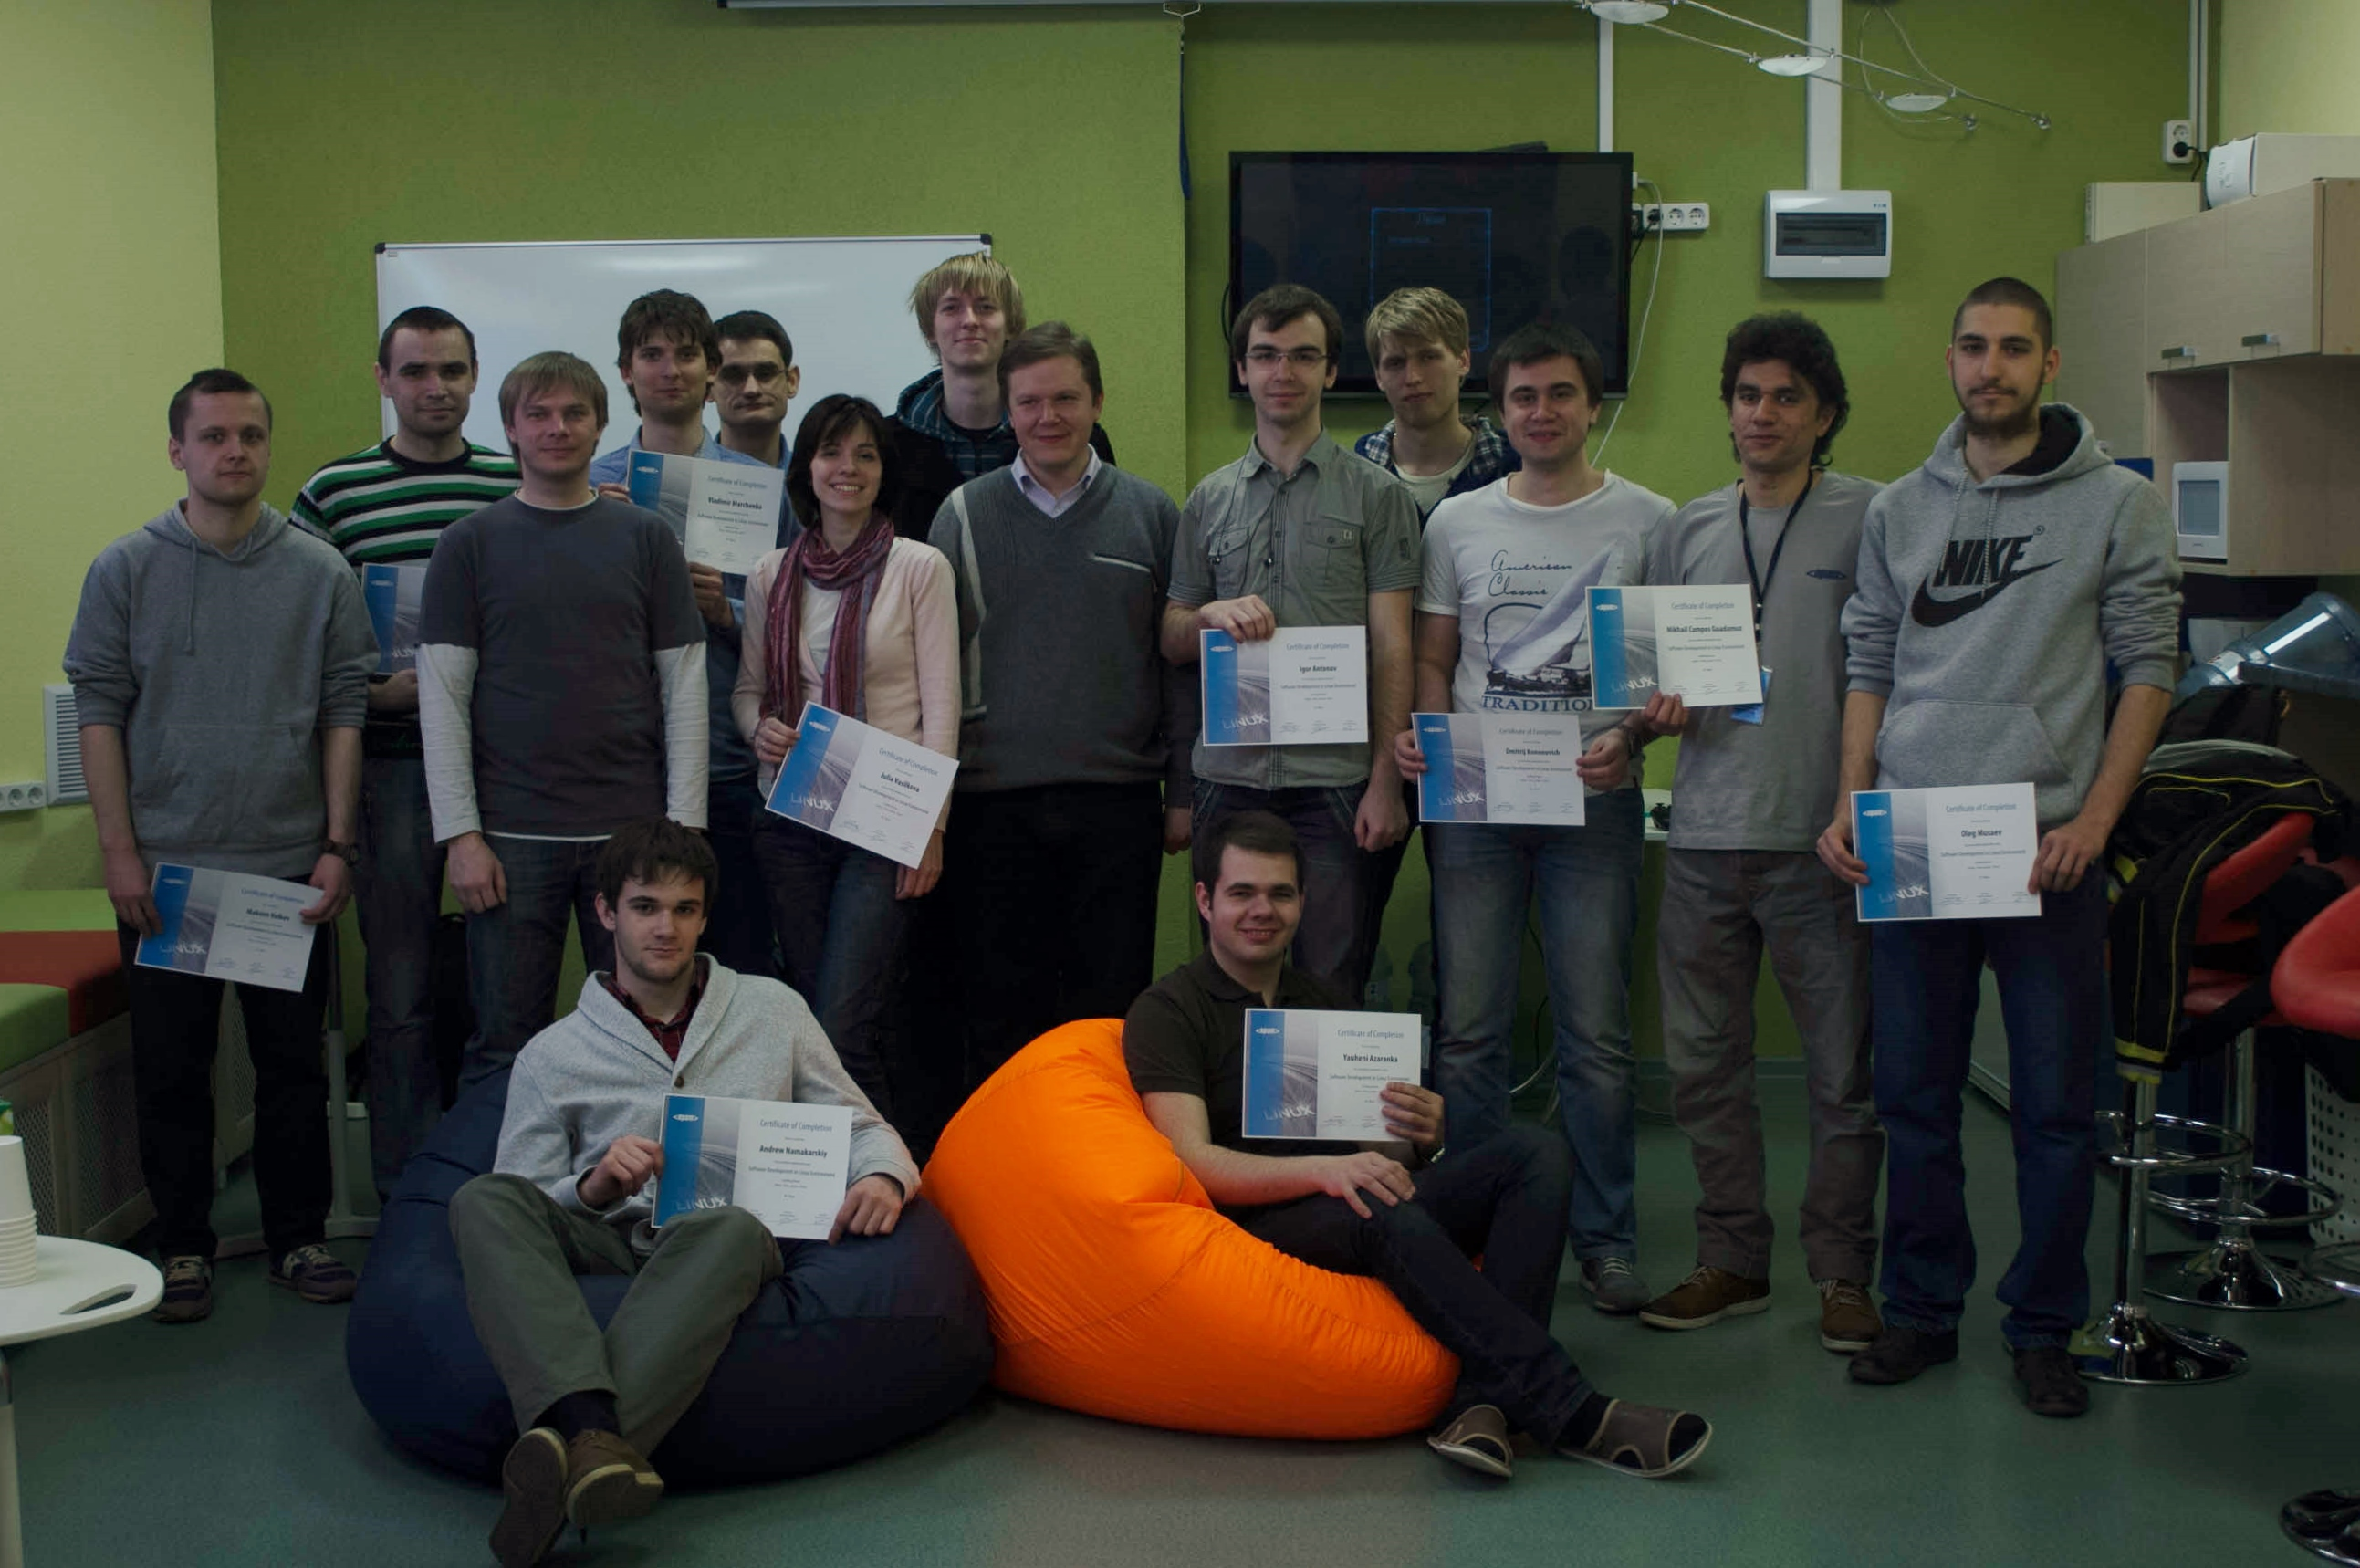
\includegraphics[width=\textwidth]{linux_courses_certificates1.jpg}
\end{frame}

\begin{frame}
  \frametitle{Анкеты и анализ}
  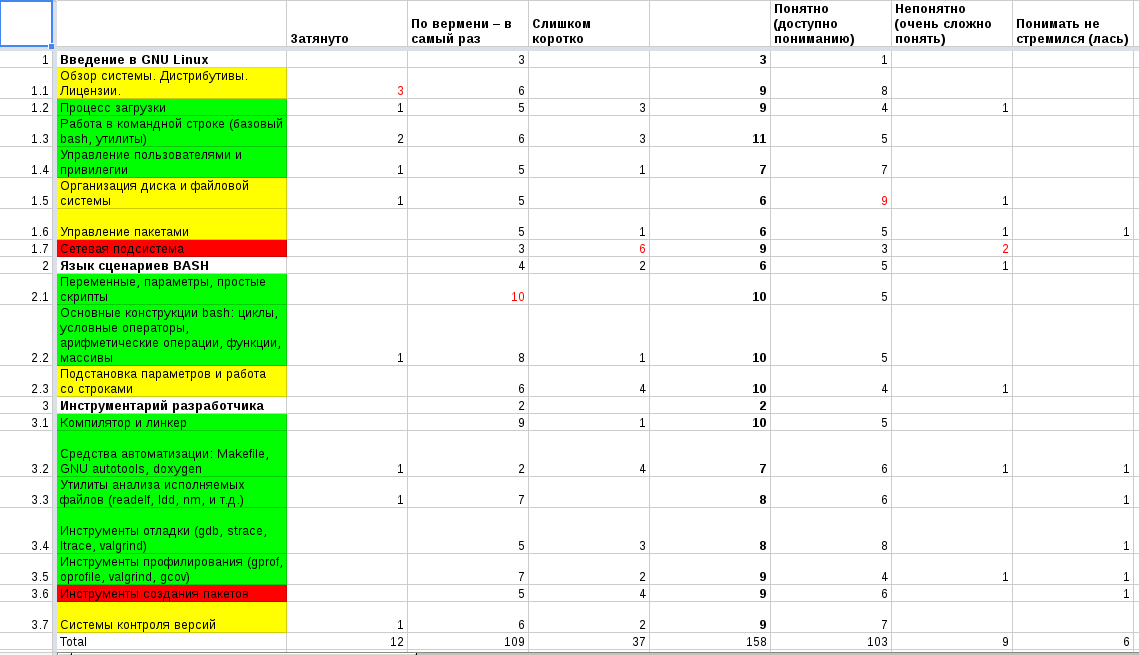
\includegraphics[width=\textwidth]{anketa.png}
\end{frame}

\subsection[2013]{Курс 2013-2014}
\begin{frame}
\frametitle{Второй набор (2013-2014)}

  \begin{columns}

  \column{0.4\textwidth}

	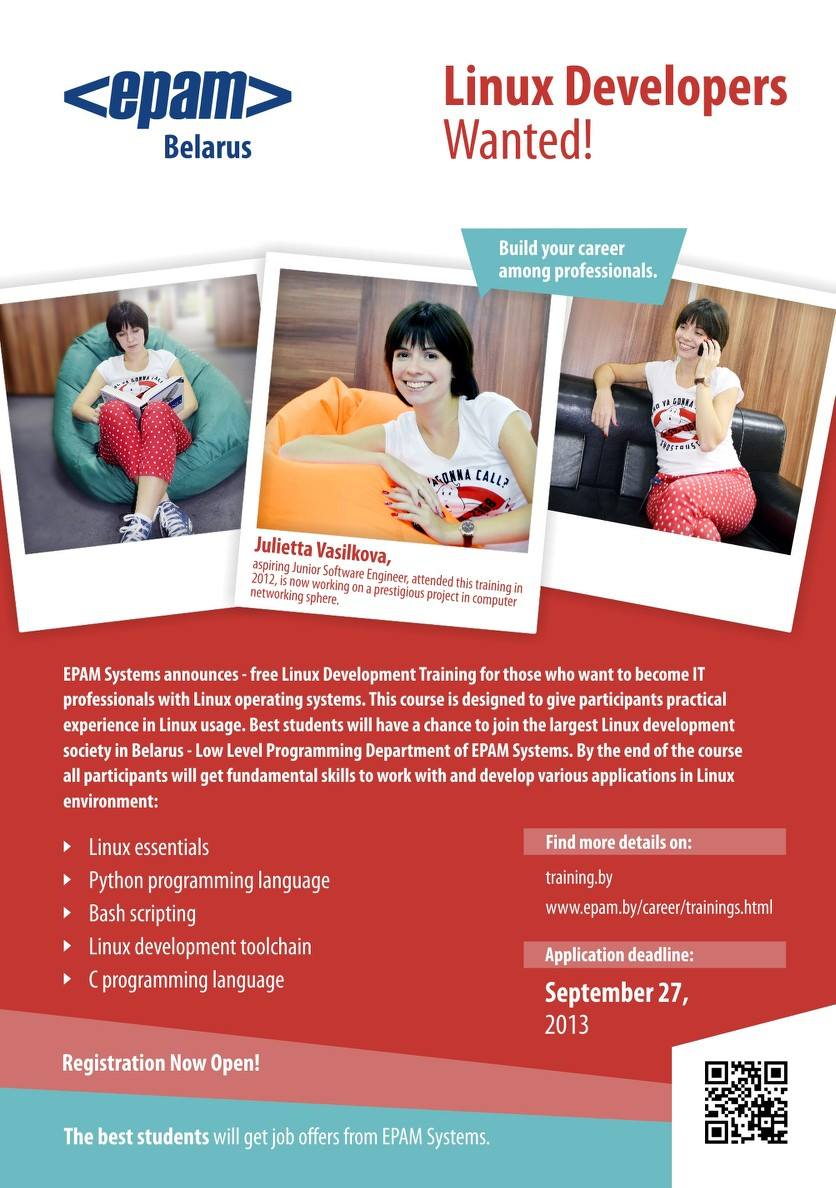
\includegraphics[width=\textwidth]{linux_courses_epam}

  \column{0.6\textwidth}
	  \begin{block}{Статистика}
		\begin{itemize}
		  \item Подано заявок: 80
		  \item Прошли телефонное интервью: 23
		  \item Дошли до курсов: 11 человек \\ + 6-8 свободных слушателей (сотрудники EPAM и не только)
		\end{itemize}
	  \end{block}
  \end{columns}
\end{frame}

\begin{frame}
\frametitle{Второй набор}
  \begin{block}{Что поменялось?}
	  \begin{itemize}
		\item Пересмотрены некоторые разделы (networking, лицензии)
		\item Добавлены новые модули
		  \begin{itemize}
	        \item C\footnote{В процессе}
			\item Python
		  \end{itemize}
		\item Еще два инструктора
	  \end{itemize}
  \end{block}
\end{frame}


\begin{frame}
  \frametitle{Неожиданные проблемы}

  \begin{block}{Конфликт интересов}


  \center{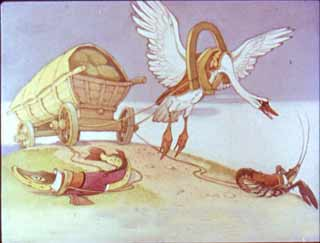
\includegraphics[width=0.3\textwidth]{Lebed_chuka_rak03.jpg}}

	\begin{columns}
		\column{0.45\textwidth}
		\begin{itemize}
			\item Введение в GNU/Linux
			\item Bash
			\item Cредства разработки, отладки и оптимизации
		\end{itemize}

		\column{0.1\textwidth}
		
		\center{\Large VS}

		\column{0.2\textwidth}
		\begin{itemize}
		  \item C
		  \item Python
		\end{itemize}
		\column{0.2\textwidth}
	\end{columns}

  \end{block}

\end{frame}
